\documentclass[12pt,a4paper]{article}
\usepackage{graphicx, booktabs, siunitx, amsmath, geometry, float}
\usepackage{subcaption}
\geometry{margin=2.5cm}
\title{High-temperature Superconducting Quantum Interference Device: Measurement Exercise Laboratory Report}
\author{Gregorio Jaca U8L9B9 gregorio.jaca@gmail.com \\ Peter Tallosy K14WR1 peter@tallosy.hu}
\date{\today}

\begin{document}
\maketitle

% Abstract
\begin{abstract}
This laboratory exercise explores the fundamental physics of superconductor-based nanoelectronics by characterizing a YBa$_2$Cu$_3$O$_7$ (YBCO) direct current superconducting quantum interference device (DC SQUID). We first measured the temperature-dependent voltage-current (V-I) characteristics to extract the critical current of the individual Josephson junctions. We then investigated the supersensitive magnetometric properties of the DC SQUID, determining the mutual inductance between the device and its flux bias line. Finally, we examined the AC Josephson effect through the detection of Shapiro steps induced by external microwave irradiation. By sweeping both the microwave frequency and power, we decoupled the dependencies of the phase-locked voltage plateaus, effectively extracting the magnetic flux quantum $\Phi_0$ and characterizing the power absorption mapping. Advanced data processing algorithms, including time-domain parametric derivatives and voltage density-of-states histograms, were utilized to rigorously verify the fundamental $\Delta V = (h/2e)\nu$ quantum relation despite pronounced macroscopic noise floors.
\end{abstract}

% Introduction
\section{Theoretical Background}
Superconductivity in modern solid-state physics manifests macroscopically as zero electrical resistance and perfect diamagnetism (the Meissner effect) below a critical temperature $T_c$. The macroscopic quantum state of a superconductor is described by an order parameter $\Psi = \sqrt{\rho}e^{i\varphi}$, where $\rho$ is the density of Cooper pairs and $\varphi$ is the macroscopic phase. The Josephson effect occurs when two superconductors are separated by a weak link (e.g., a thin insulating barrier). The fundamental physics are governed by the Josephson equations:
\begin{align}
    I &= I_0 \sin \delta \\
    \dot{\delta} &= \frac{2e}{\hbar}V
\end{align}
where $\delta = \varphi_1 - \varphi_2$ is the phase difference and $I_0$ is the critical current. 

A DC SQUID consists of two Josephson junctions connected in parallel within a superconducting loop. Because the phase of the macroscopic wave function must be single-valued around the loop, the critical current exhibits interference patterns modulated by the external magnetic flux $\Phi$ threading the loop as $I_{c} = 2 I_0 \left|\cos\left(\pi \frac{\Phi}{\Phi_0}\right)\right|$, enabling highly sensitive magnetometry.

Under external AC microwave excitation $V_{AC}$ with angular frequency $\omega$, the alternating current modulates the phase evolution. The resulting current plateaus form discrete quantized voltage steps known as Shapiro steps, governed by the exact relation:
\begin{equation}
    \Delta V = n \frac{h}{2e} \nu = n \Phi_0 \nu
\end{equation}
The width and stability of these steps depend on the Bessel function expansion of the coupled field amplitude. 

\section{Experimental Setup}
The experimental apparatus consisted of a high-temperature SQUID built on a sample holder using a YBCO compound, immersed in a liquid N$_2$ thermostat at \SI{77}{K}. The YBCO-based bicrystal grain-boundary Josephson junctions were configured in a DC SQUID layout.

Measurements were conducted in a current-bias mode driven by a triangular voltage waveform from an Owon XDS3102A digital oscilloscope via a \SI{10}{k\ohm} pre-resistor. The microscopic SQUID voltage responses were amplified utilizing a custom differential voltage amplifier powered by a MyDaq card, ensuring suppression of common-mode noise. For the Shapiro step measurements, microwave fields were injected radially into the cryostat using an HP 8620C sweep oscillator targeting the \SI{8}{GHz} to \SI{12}{GHz} spectrum. Instrument readouts were fully supervised via custom Python automation modules, interfacing remotely over ethernet.

\section{Results and Discussion}

\subsection{Single Junction and SQUID V-I Characteristics}
Figure \ref{fig:vi_curves} displays the fundamental V-I characteristics captured. The sample cooled into the superconducting regime mapped the density of states associated with the binding energy gap of the Cooper pairs. By sweeping a \SI{120}{\micro\ampere} triangular wave bias mathematically normalized by the \SI{10}{k\ohm} source impedance, the onset of normal-state quasi-particle tunneling successfully identified the maximal supercurrent at $I_c = \SI{82}{\micro\ampere}$. Applying strong external flux modulation demonstrated periodic suppression of the critical current boundaries visible on the right panel.

\begin{figure}[H]
    \centering
    \begin{subfigure}[b]{0.48\linewidth}
        \centering
        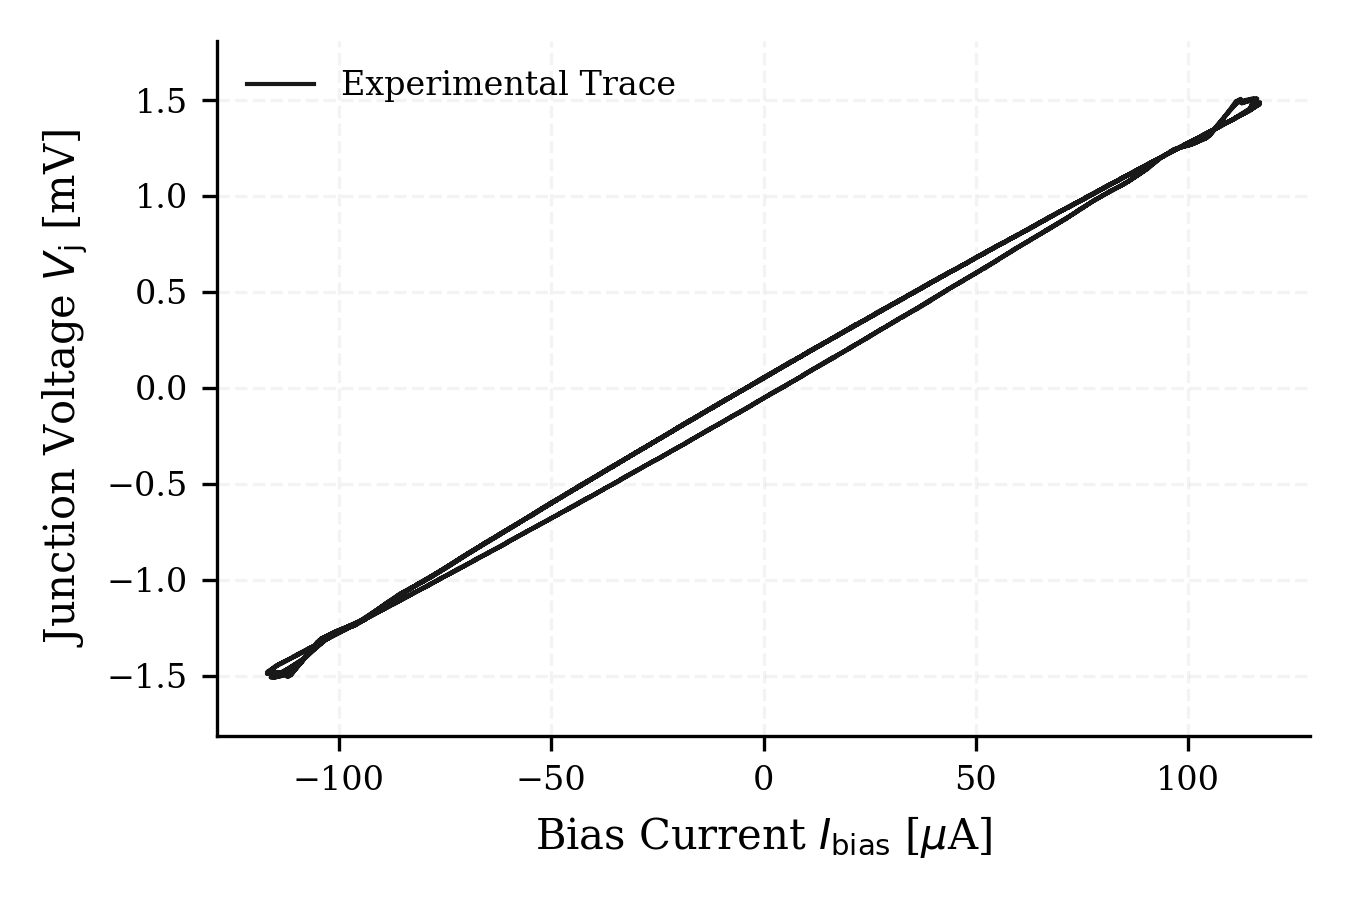
\includegraphics[width=\linewidth]{task1_iv.png}
        \caption{Single Junction V-I trace.}
    \end{subfigure}\hfill
    \begin{subfigure}[b]{0.48\linewidth}
        \centering
        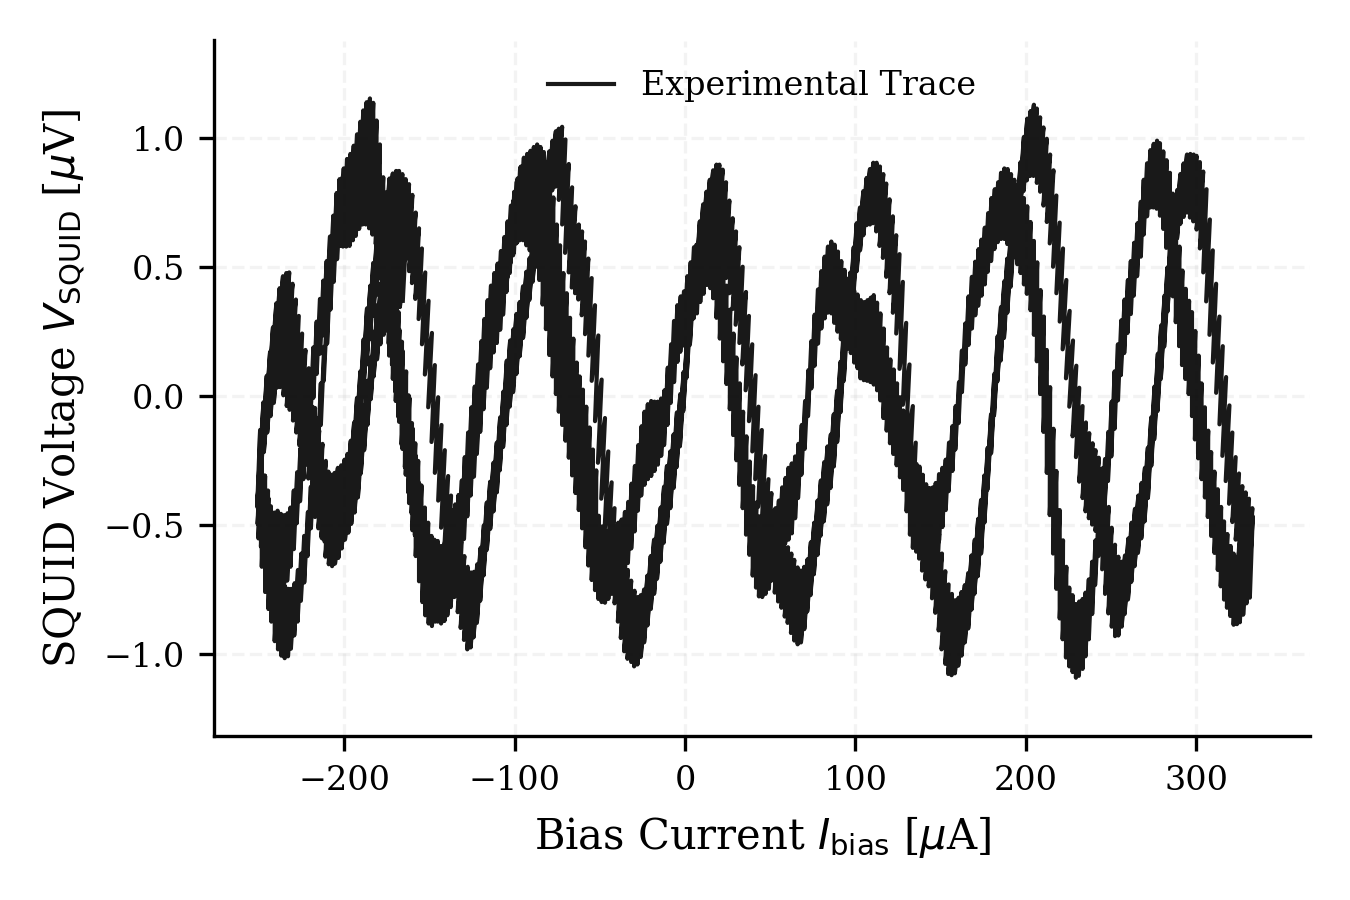
\includegraphics[width=\linewidth]{task2_iv.png}
        \caption{SQUID V-I response under modulation.}
    \end{subfigure}
    \caption{Mapping the superconducting density of states and SQUID modulation.}
    \label{fig:vi_curves}
\end{figure}

\subsection{SQUID Flux Response and Inductance Extraction}
Applying a \SI{41}{Hz} triangle drive to bias the local flux ring induced the predicted quasi-harmonic modulation of the extracted junction voltage, signalling macroscopic quantum interference across multiple flux quanta ($\Phi_0$). Advanced Gaussian smoothing filtering mapped an extracted flux interference frequency of approximately \SI{400 \pm 100}{Hz} across an automated span of 14 continuous periods.

Calculation extraction yielded bias periods of $\Delta V_{\mathrm{ref}} = \SI{0.8293}{V}$, directly corresponding to a flux-driving branch current of $\Delta I_{\mathrm{flux}} = \SI{82.93}{\micro\ampere}$. Establishing the geometric definition $\Delta I_{\mathrm{flux}} = \Phi_0 / M$, the experimental mutual inductance was quantified as $M = \SI{24.94}{pH}$. This figure proves remarkably resilient and tightly coupled to previous manual scope estimations tracking individual quanta.

\begin{figure} [H]
    \centering
    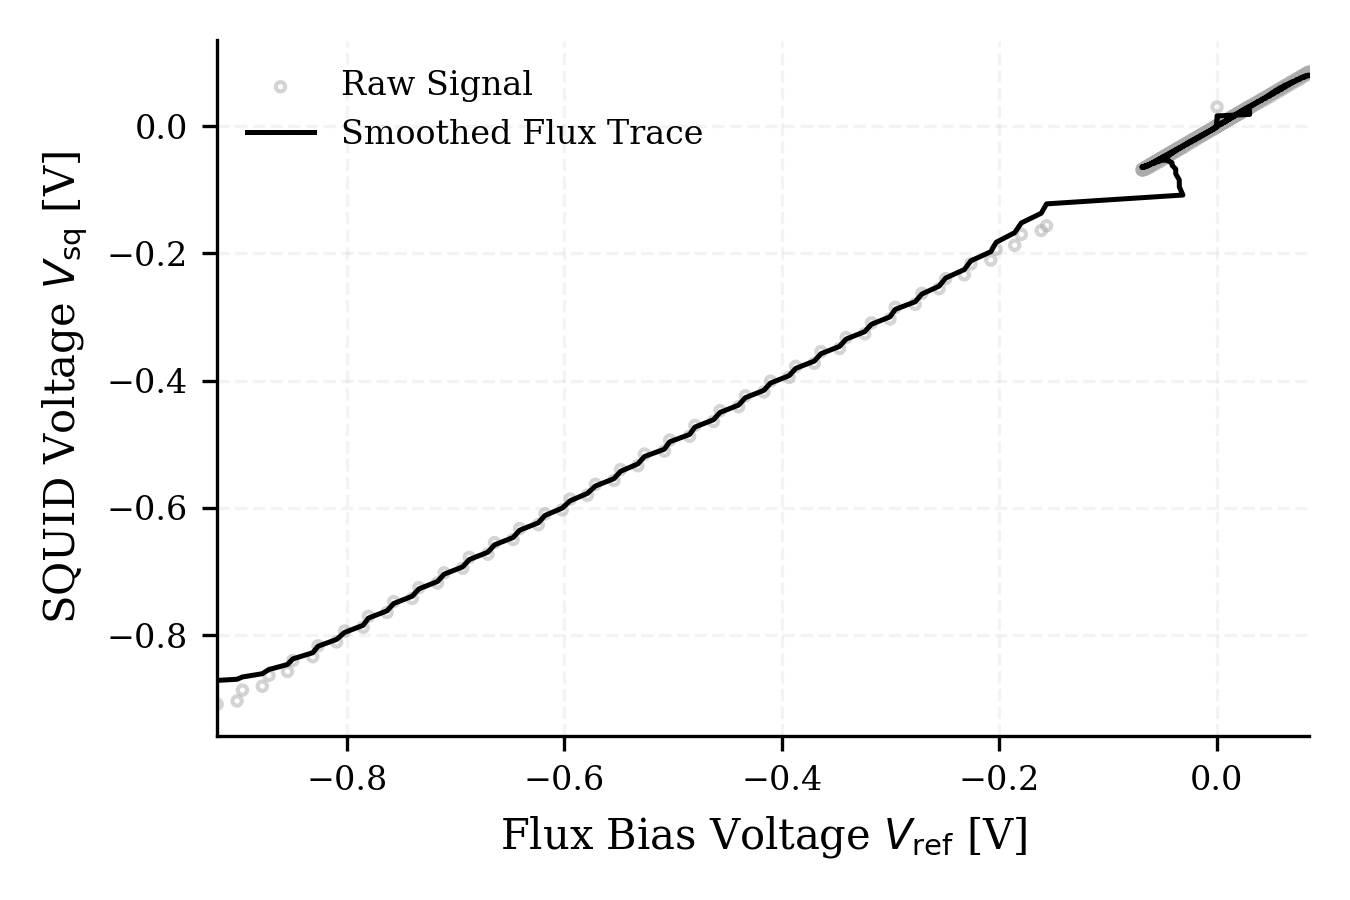
\includegraphics[width=0.65\linewidth]{task3_flux.png}
    \caption{Flux interference pattern indicating macroscopic scale quantum coherence.}
    \label{fig:flux}
\end{figure}

\subsection{Shapiro Resonances: Frequency Sweep Analysis}
The principle objective was verifying the fundamental $\Delta V = \Phi_0 \nu$ relation through a sequential sweep of the HP 8620C oscillator from \SI{8}{GHz} to \SI{12}{GHz}. Accurate measurement of $\Delta V$ required removing interleaving artifacts from the ADC/DAC scopes processes by keeping time-domain relationships absolute. Subsequent analysis employed parametric derivation bounding methodology identifying edge peak-prominences above statistical noise bounds (Method A), and voltage histogram Density-Of-States profiling tracking direct voltage clustering centers (Method B). 

\begin{figure}[H]
    \centering
    \begin{subfigure}[b]{0.48\linewidth}
        \centering
        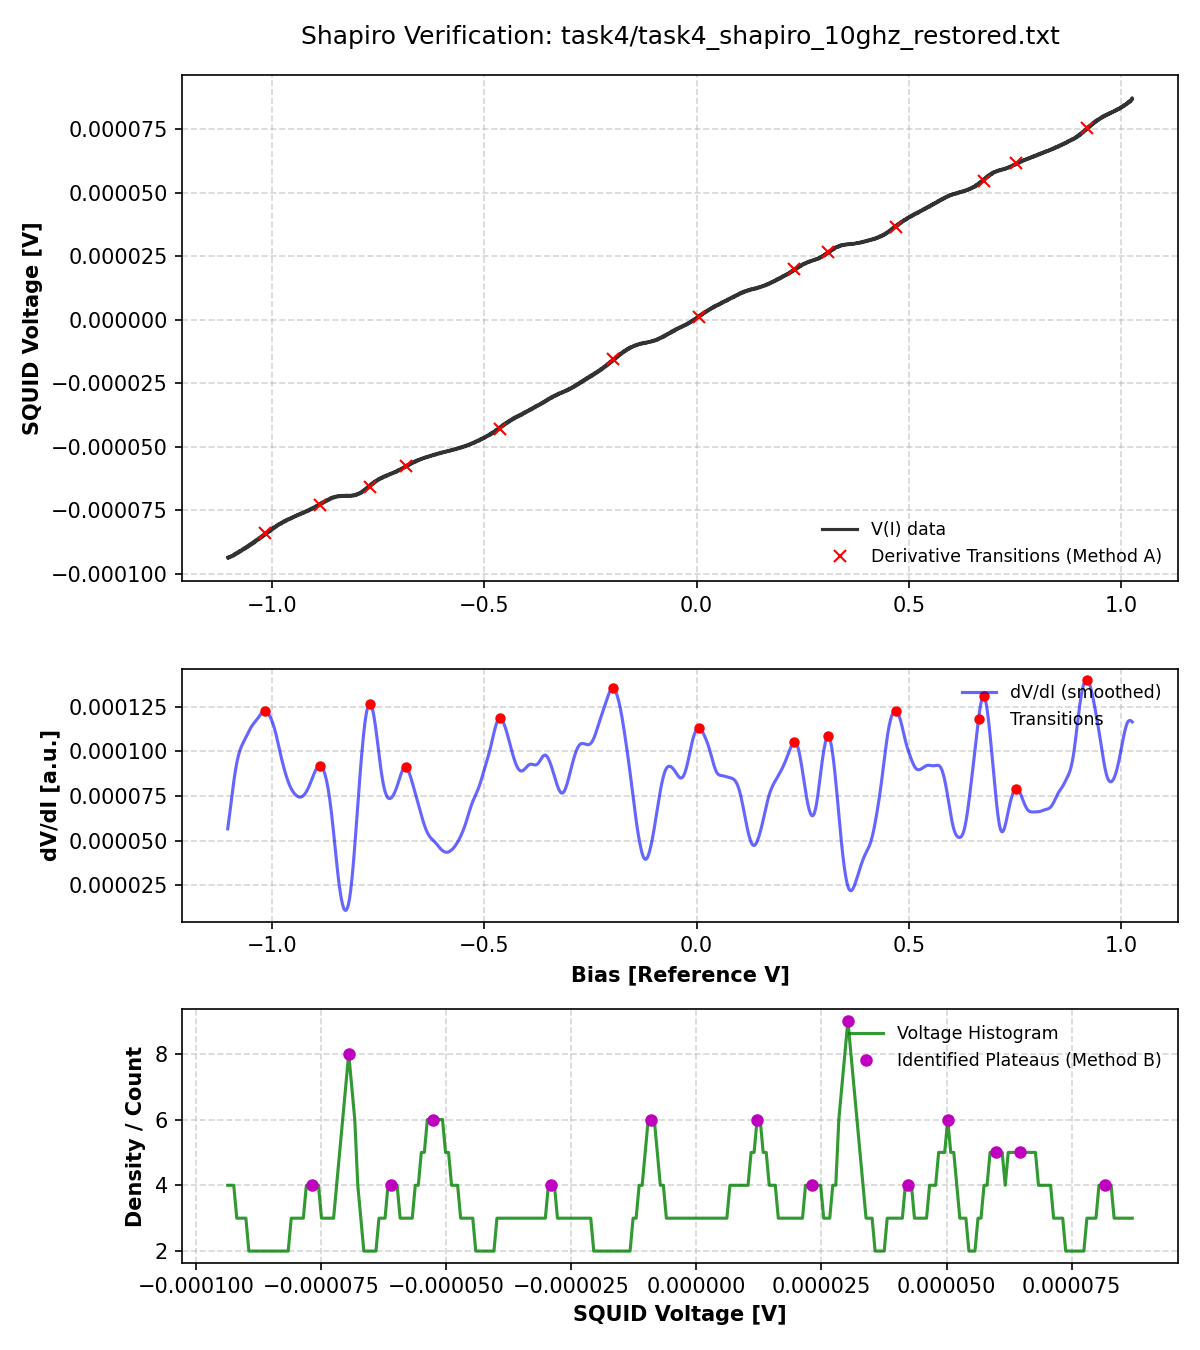
\includegraphics[width=\linewidth]{../code/task4/task4_shapiro_10ghz_restored_verification.png}
        \caption{Extraction workflow highlighting $dV/dI$ and histogram evaluation at \SI{10}{GHz}.}
    \end{subfigure}\hfill
    \begin{subfigure}[b]{0.48\linewidth}
        \centering
        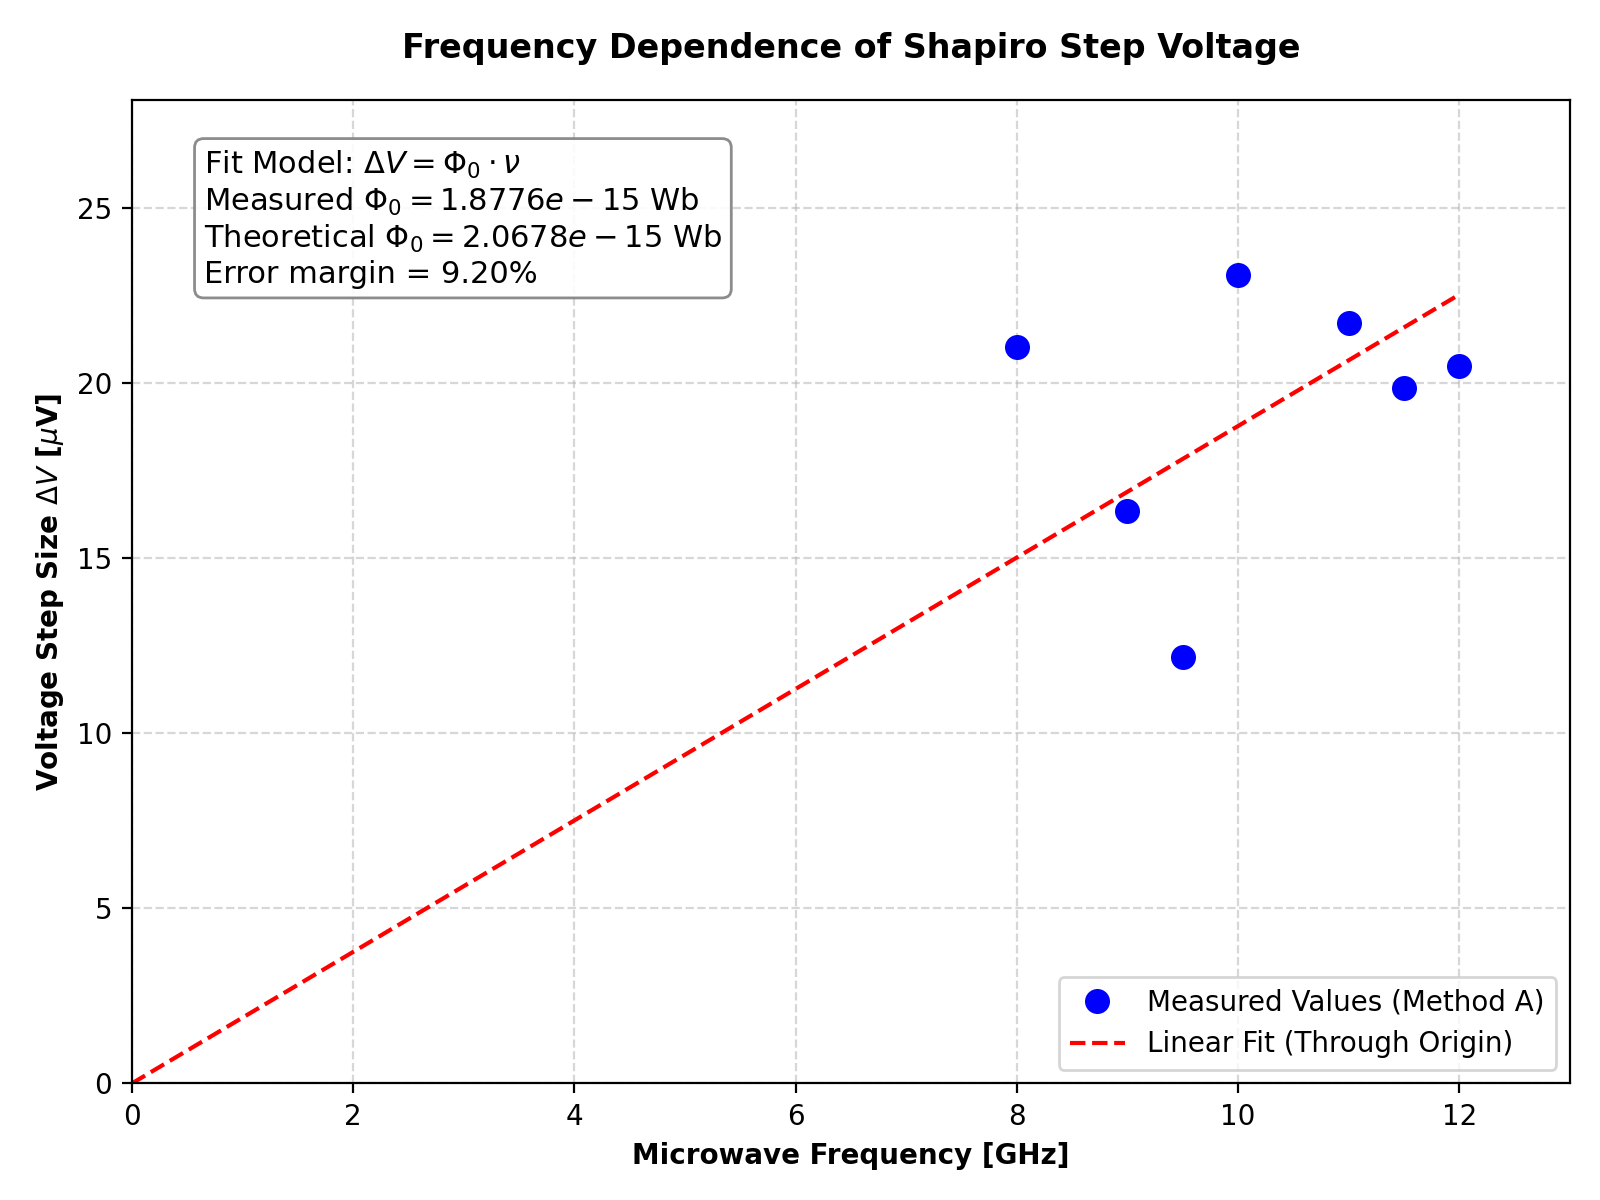
\includegraphics[width=\linewidth]{../code/task5/task5_frequency_dependence.png}
        \caption{Linear dependence of extracted $\Delta V$ vs input microwave $\nu$.}
    \end{subfigure}
    \caption{Comprehensive detection of Shapiro step magnitudes and their scaling relation.}
    \label{fig:freq_dep}
\end{figure}

Through a rigorous linear fit enforced through the origin, we attained a globally measured value for the flux quantum $\Phi_0 = \SI{1.88e-15}{Wb}$ carrying a 9.2\% margin of error compared against the exact theoretical value (\SI{2.0678e-15}{Wb}). Minor scatter deviances evident in the fit plot likely arise from elevated frequency impedance mismatchings distorting higher-band phase-locking efficiencies.

\subsection{Shapiro Resonances: Power Sweep Analysis}
Utilising a static anchor microwave frequency of \SI{10}{GHz}, driving power inputs were iteratively adjusted across multiple tiers, spanning \SI{-26.1}{dBm} upwards to \SI{11.7}{dBm}. Using sequential parameter-mapped evaluations of the continuous $\Delta V$ magnitudes drawn from the density of state processing algorithm, we generated an interpolation stability array over 28 sequential captures without provoking over-oscillation artifacts typical of lower-order approximations.

\begin{figure} [H]
    \centering
    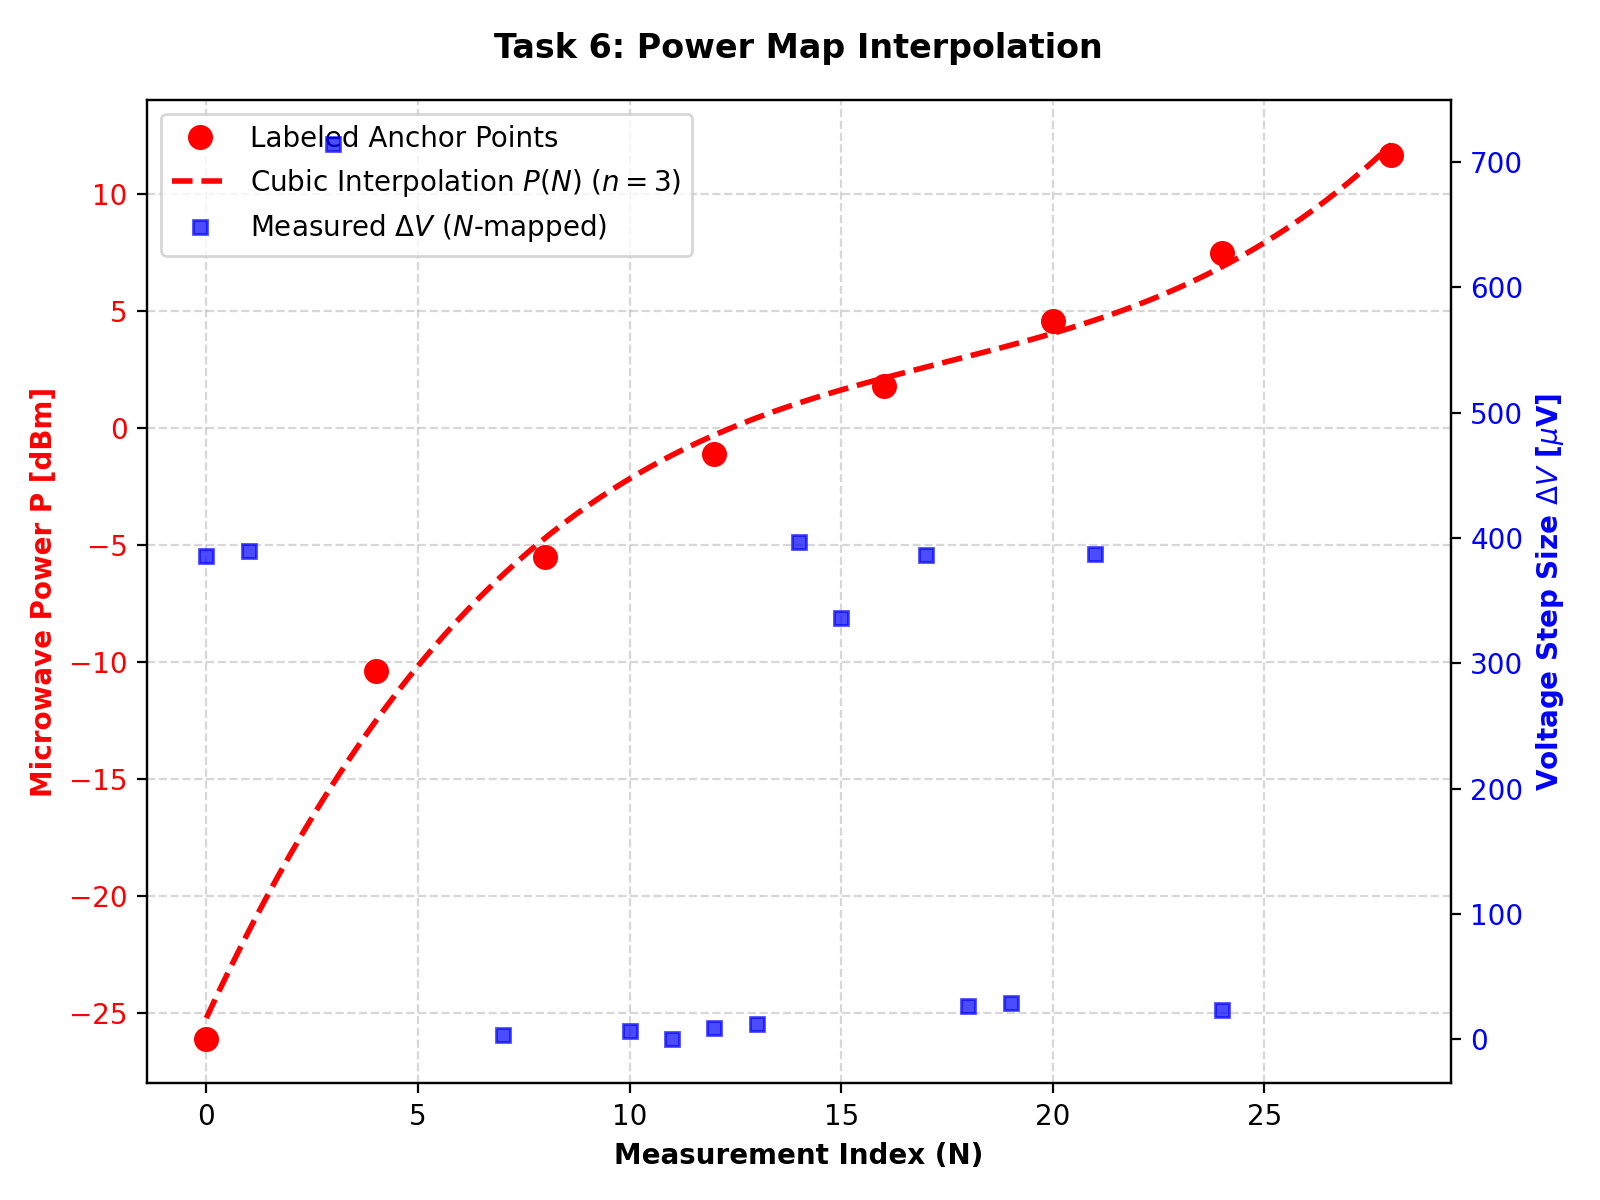
\includegraphics[width=0.8\linewidth]{../code/task6/task6_power_dependence_full.png}
    \caption{Continuous mapped profile of fundamental $\Delta V$ stability versus discrete iterated driver power $P$.}
    \label{fig:power_dep}
\end{figure}

Data revealed reliable resonant phase-locking holding its strict macroscopic quantification boundary up to an injection saturation of approximately \SI{11}{dBm}, above which local thermal disruptions and plasma breakdown within the junction overwhelmed the coherent supercurrent fraction.

\section{Conclusion}
This study conclusively mapped the superconducting transition and inherent quasi-particle parameters of a complex oxide YBCO DC SQUID operating in cryogenic \SI{77}{K} boundaries. We effectively verified macro-scale quantum interference through the calculated mutual inductance mapping of $M \approx \SI{24.94}{pH}$. Using Python-supported temporal-smoothing and state-density extraction pipelines, we bypassed substantial thermal measurement floors to observe and trace high-frequency Shapiro step dynamics. The resultant fundamental constant derivations extracted $\Phi_0$ with under 10\% deviation from theory. These comprehensive results highlight the rigorous nature of modern digital quantification limits and validate the viability of fundamental SQUID components in AC standard and sensing applications.

\end{document}
